% t-SNE Lecture - Slides 1-9 (Revised Slide 8 for aesthetics)
\documentclass{beamer}
\usetheme{Madrid}
\usecolortheme{seahorse}
\usepackage{amsmath}
\usepackage{amssymb}
\usepackage{graphicx}
\usepackage{tikz}
\usetikzlibrary{shapes.geometric, arrows.meta, positioning}

% Define custom colors for consistency
\definecolor{upcblue}{RGB}{0,123,199}
\definecolor{upcgray}{RGB}{100,100,100}
\definecolor{highlight}{RGB}{255,127,0}

% Adjust beamer margins to prevent truncation
\setbeamersize{text margin left=5mm,text margin right=5mm}

\begin{document}

% SLIDE 1: Title Slide
\begin{frame}[plain]
\vspace{0.5cm}
\begin{center}
{\LARGE \textcolor{upcblue}{\textbf{Nonlinear Dimensionality Reduction:}}}\\[0.2cm]
{\huge \textcolor{upcblue}{\textbf{t-Stochastic Neighbor Embedding}}}\\[0.2cm]
{\huge \textcolor{upcblue}{\textbf{(t-SNE)}}}\\[1cm]

{\large \textbf{Prof. Endri Raco}}\\[0.2cm]
{\normalsize Polytechnic University of Tirana}\\[0.1cm]
{\small \textit{Erasmus+ Exchange Professor}}\\[0.8cm]

{\large \textcolor{upcgray}{Advanced Multivariate Analysis}}\\[0.2cm]
{\normalsize Polytechnic University of Catalonia (UPC)}\\[0.3cm]
{\normalsize October 15, 2025}
\end{center}

\vspace{0.3cm}
\begin{center}
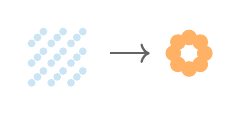
\begin{tikzpicture}[scale=0.25]
% 3D point cloud on the left
\foreach \x in {0,1,2}
    \foreach \y in {0,1,2}
        \foreach \z in {0,1,2}
            \node[circle, fill=upcblue!20, inner sep=1pt] at (\x+\z*0.3,\y+\z*0.3) {};
            
% Arrow indicating transformation
\draw[->, thick, upcgray] (4,1.5) -- (6,1.5);

% 2D circular arrangement on the right
\foreach \angle in {0,45,...,315}
    \node[circle, fill=highlight!60, inner sep=2pt] at ({8+0.8*cos(\angle)},{1.5+0.8*sin(\angle)}) {};
\end{tikzpicture}
\end{center}
\end{frame}

% SLIDE 2: Welcome and Overview
\begin{frame}{Welcome to Advanced Multivariate Analysis}
\vspace{-0.2cm}
{\color{upcblue}\textbf{Today's Journey}}\\[0.2cm]
\begin{itemize}
    \setlength\itemsep{0.3em}
    \item \textbf{2-hour deep dive} into t-SNE
    \item \textbf{Mathematical foundations} to practical insights
    \item \textbf{Three key parts:}
    \begin{enumerate}
        \item SNE - The original idea
        \item t-SNE - Solving the crowding problem  
        \item Hyperparameters \& interpretation
    \end{enumerate}
\end{itemize}

\vspace{0.3cm}
\begin{center}
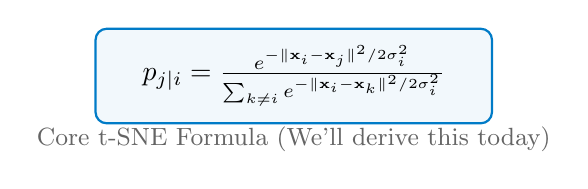
\begin{tikzpicture}[scale=0.8]
    \node[draw=upcblue, thick, rounded corners, 
          minimum width=5cm, minimum height=1.2cm,
          fill=upcblue!5] at (0,0) {
        \begin{minipage}{4.8cm}
        \centering
        $p_{j|i} = \frac{e^{-\|\mathbf{x}_i - \mathbf{x}_j\|^2/2\sigma_i^2}}{\sum_{k \neq i} e^{-\|\mathbf{x}_i - \mathbf{x}_k\|^2/2\sigma_i^2}}$
        \end{minipage}
    };
    \node at (0,-1) {\small \textcolor{upcgray}{Core t-SNE Formula (We'll derive this today)}};
\end{tikzpicture}
\end{center}
\end{frame}

% SLIDE 3: The Challenge of High-Dimensional Data
\begin{frame}{The Curse of Dimensionality}
\vspace{-0.3cm}
\begin{columns}[T]
\begin{column}{0.48\textwidth}
\textbf{\color{upcblue}Our Intuition Works Here:}

\begin{center}
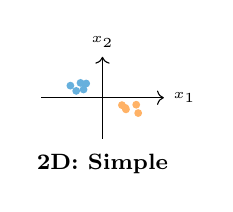
\begin{tikzpicture}[scale=0.65]
    % 2D scatter plot
    \node at (0,-1.3) {\footnotesize \textbf{2D: Simple}};
    \draw[->] (-1.2,0) -- (1.2,0) node[right] {\tiny $x_1$};
    \draw[->] (0,-0.8) -- (0,0.8) node[above] {\tiny $x_2$};
    
    % Cluster 1
    \foreach \i in {1,...,5} {
        \node[circle, fill=upcblue!60, inner sep=1pt] at ({-0.5+0.2*rand},{0.3+0.2*rand}) {};
    }
    % Cluster 2
    \foreach \i in {1,...,5} {
        \node[circle, fill=highlight!60, inner sep=1pt] at ({0.5+0.2*rand},{-0.3+0.2*rand}) {};
    }
\end{tikzpicture}
\end{center}

\begin{center}
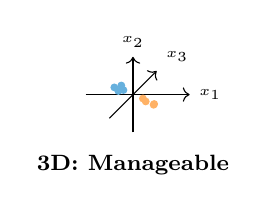
\begin{tikzpicture}[scale=0.6]
    % 3D scatter plot
    \node at (0,-1.5) {\footnotesize \textbf{3D: Manageable}};
    \draw[->] (-1,0) -- (1.2,0) node[right] {\tiny $x_1$};
    \draw[->] (0,-0.8) -- (0,0.8) node[above] {\tiny $x_2$};
    \draw[->] (-0.5,-0.5) -- (0.5,0.5) node[above right] {\tiny $x_3$};
    
    % 3D clusters
    \foreach \i in {1,...,4} {
        \node[circle, fill=upcblue!60, inner sep=1pt] at ({-0.3+0.15*rand},{0.2+0.15*rand}) {};
    }
    \foreach \i in {1,...,4} {
        \node[circle, fill=highlight!60, inner sep=1pt] at ({0.3+0.15*rand},{-0.2+0.15*rand}) {};
    }
\end{tikzpicture}
\end{center}
\end{column}

\begin{column}{0.48\textwidth}
\textbf{\color{upcblue}But Not Here:}

\begin{center}
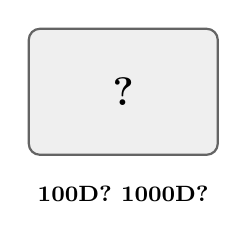
\begin{tikzpicture}
    \draw[upcgray, thick, rounded corners, fill=upcgray!10] 
          (-1.2,-0.8) rectangle (1.2,0.8);
    \node at (0,0) {\Large \textbf{?}};
    \node at (0,-1.3) {\footnotesize \textbf{100D? 1000D?}};
\end{tikzpicture}
\end{center}

\vspace{0.3cm}
\textcolor{upcgray}{\textbf{Problems:}}
\begin{itemize}
    \small
    \item \textcolor{highlight}{Distance concentration}
    \item \textcolor{highlight}{Volume:} $V_n(r) \propto r^n$
    \item \textcolor{highlight}{Sparse data}
\end{itemize}

\vspace{0.2cm}
\centering
\small\textit{\color{upcblue}``Geometric intuition fails''}
\end{column}
\end{columns}
\end{frame}

% SLIDE 4: Why Reduce Dimensions?
\begin{frame}{Goals of Dimensionality Reduction}
\vspace{-0.3cm}
\begin{columns}[T]
\begin{column}{0.48\textwidth}
\textbf{\color{upcblue}Goal 1: Visualization}

\begin{center}
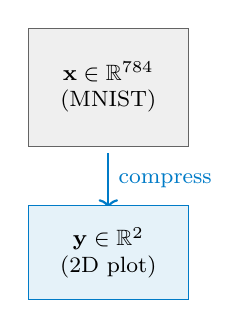
\begin{tikzpicture}[scale=0.7]
    % High-dimensional
    \node[draw=upcgray, minimum width=2cm, minimum height=1.5cm, fill=upcgray!10] 
          at (0,0) {
        \begin{minipage}{1.8cm}
        \centering
        \footnotesize
        $\mathbf{x} \in \mathbb{R}^{784}$\\
        (MNIST)
        \end{minipage}
    };
    
    % Arrow
    \draw[->, thick, upcblue] (0,-1.2) -- (0,-2.2) 
          node[midway, right] {\footnotesize compress};
    
    % Low-dimensional
    \node[draw=upcblue, minimum width=2cm, minimum height=1.2cm, fill=upcblue!10] 
          at (0,-3) {
        \begin{minipage}{1.8cm}
        \centering
        \footnotesize
        $\mathbf{y} \in \mathbb{R}^{2}$\\
        (2D plot)
        \end{minipage}
    };
\end{tikzpicture}
\end{center}

\small
\textcolor{upcgray}{\textbf{Key:}} ``See'' hidden structure
\end{column}

\begin{column}{0.48\textwidth}
\textbf{\color{upcblue}Goal 2: Feature Extraction}

\begin{center}
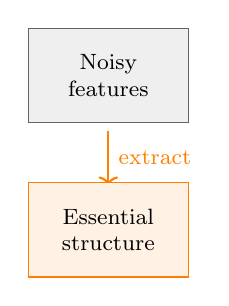
\begin{tikzpicture}[scale=0.7]
    % Original
    \node[draw=upcgray, minimum width=2cm, minimum height=1.2cm, fill=upcgray!10] 
          at (0,0) {
        \begin{minipage}{1.8cm}
        \centering
        \footnotesize
        Noisy\\features
        \end{minipage}
    };
    
    % Arrow
    \draw[->, thick, highlight] (0,-1) -- (0,-2) 
          node[midway, right] {\footnotesize extract};
    
    % Essential
    \node[draw=highlight, minimum width=2cm, minimum height=1.2cm, fill=highlight!10] 
          at (0,-2.8) {
        \begin{minipage}{1.8cm}
        \centering
        \footnotesize
        Essential\\structure
        \end{minipage}
    };
\end{tikzpicture}
\end{center}

\small
\textcolor{upcgray}{\textbf{Benefits:}}
\begin{itemize}
    \footnotesize
    \item Noise reduction
    \item Efficiency
    \item Better ML
\end{itemize}
\end{column}
\end{columns}

\vspace{0.3cm}
\begin{center}
\colorbox{upcblue!10}{
\begin{minipage}{0.85\textwidth}
\centering
\small\textbf{Challenge:} Preserve relationships while reducing dimensions
\end{minipage}
}
\end{center}
\end{frame}

% SLIDE 5: The Limits of Linear Projections
\begin{frame}{When Linear Methods Falter}
\vspace{-0.3cm}
\begin{columns}[T]
\begin{column}{0.48\textwidth}
\textbf{\color{upcblue}Swiss Roll Dataset}

\begin{center}
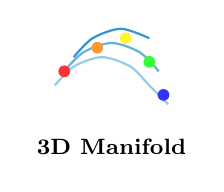
\begin{tikzpicture}[scale=0.6]
    % Swiss Roll curves
    \draw[thick, upcblue!40] plot[smooth, tension=0.5] 
          coordinates {(-1.2,0) (-0.8,0.4) (-0.2,0.6) (0.4,0.4) (0.8,0) (1.2,-0.4)};
    \draw[thick, upcblue!60] plot[smooth, tension=0.5] 
          coordinates {(-1,0.3) (-0.6,0.7) (0,0.9) (0.6,0.7) (1,0.3)};
    \draw[thick, upcblue!80] plot[smooth, tension=0.5] 
          coordinates {(-0.8,0.6) (-0.4,1) (0.2,1.2) (0.8,1)};
    
    % Points with colors
    \node[circle, fill=red!80, inner sep=1.5pt] at (-1,0.3) {};
    \node[circle, fill=orange!80, inner sep=1.5pt] at (-0.3,0.8) {};
    \node[circle, fill=yellow!80, inner sep=1.5pt] at (0.3,1) {};
    \node[circle, fill=green!80, inner sep=1.5pt] at (0.8,0.5) {};
    \node[circle, fill=blue!80, inner sep=1.5pt] at (1.1,-0.2) {};
    
    \node at (0,-1.3) {\footnotesize \textbf{3D Manifold}};
\end{tikzpicture}
\end{center}

\small
\textcolor{upcgray}{\textbf{True Structure:}}\\
\footnotesize 2D manifold in 3D space
\end{column}

\begin{column}{0.48\textwidth}
\textbf{\color{upcblue}PCA Projection}

\begin{center}
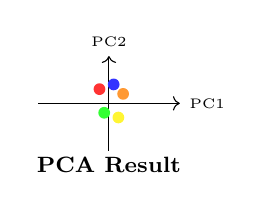
\begin{tikzpicture}[scale=0.6]
    % PCA axes
    \draw[->] (-1.5,0) -- (1.5,0) node[right] {\tiny PC1};
    \draw[->] (0,-1) -- (0,1) node[above] {\tiny PC2};
    
    % Mixed colors - PCA failure
    \node[circle, fill=red!80, inner sep=1.5pt] at (-0.2,0.3) {};
    \node[circle, fill=blue!80, inner sep=1.5pt] at (0.1,0.4) {};
    \node[circle, fill=orange!80, inner sep=1.5pt] at (0.3,0.2) {};
    \node[circle, fill=green!80, inner sep=1.5pt] at (-0.1,-0.2) {};
    \node[circle, fill=yellow!80, inner sep=1.5pt] at (0.2,-0.3) {};
    
    \node at (0,-1.3) {\footnotesize \textbf{PCA Result}};
\end{tikzpicture}
\end{center}

\small
\textcolor{highlight}{\textbf{Problem:}}\\
\footnotesize Preserves variance,\\
\footnotesize destroys local structure
\end{column}
\end{columns}

\vspace{0.2cm}
\begin{center}
\colorbox{highlight!20}{
\begin{minipage}{0.85\textwidth}
\centering
\small\textit{Need methods that preserve \textbf{local relationships}}
\end{minipage}
}
\end{center}
\end{frame}

% SLIDE 6: The Manifold Hypothesis
\begin{frame}{The Manifold Hypothesis}
\vspace{-0.3cm}
\begin{center}
\colorbox{upcblue!10}{
\begin{minipage}{0.9\textwidth}
\centering
\textit{``High-dimensional data often lies on or near}\\
\textit{a much lower-dimensional manifold''}
\end{minipage}
}
\end{center}

\vspace{0.3cm}
\begin{columns}[T]
\begin{column}{0.48\textwidth}
\textbf{\color{upcblue}Example: Earth's Surface}

\begin{center}
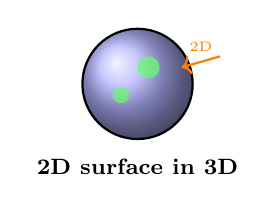
\begin{tikzpicture}[scale=0.7]
    % Earth sphere
    \shade[ball color=blue!30] (0,0) circle (1cm);
    \draw[thick] (0,0) circle (1cm);
    
    % Continents
    \fill[green!60, opacity=0.7] (0.2,0.3) circle (0.2cm);
    \fill[green!60, opacity=0.7] (-0.3,-0.2) circle (0.15cm);
    
    % Arrow
    \draw[->, thick, highlight] (1.5,0.5) -- (0.8,0.3) 
          node[above, midway] {\tiny 2D};
    
    \node at (0,-1.5) {\footnotesize \textbf{2D surface in 3D}};
\end{tikzpicture}
\end{center}
\end{column}

\begin{column}{0.48\textwidth}
\textbf{\color{upcblue}Mathematical Form}

\small
Data: $\mathbf{X} = \{\mathbf{x}_1, ..., \mathbf{x}_n\}$\\
where $\mathbf{x}_i \in \mathbb{R}^D$

\vspace{0.2cm}
\textbf{Assumption:}\\
$\exists$ manifold $\mathcal{M}$ with dim $d \ll D$:

$$\mathbf{x}_i \approx f(\mathbf{z}_i) + \epsilon_i$$

\footnotesize
\begin{itemize}
    \item $\mathbf{z}_i \in \mathbb{R}^d$ (low-dim)
    \item $f: \mathbb{R}^d \rightarrow \mathbb{R}^D$
    \item $\epsilon_i$ (noise)
\end{itemize}
\end{column}
\end{columns}

\vspace{0.2cm}
\begin{center}
\colorbox{upcgray!10}{
\begin{minipage}{0.85\textwidth}
\centering
\small\textbf{Goal:} Uncover this hidden low-dimensional structure
\end{minipage}
}
\end{center}
\end{frame}

% SLIDE 7: A Glimpse of t-SNE
\begin{frame}{Preserving Neighborhoods: t-SNE in Action}
\vspace{-0.2cm}
\begin{columns}[T]
\begin{column}{0.48\textwidth}
\textbf{\color{upcblue}PCA on MNIST Digits}

\begin{center}
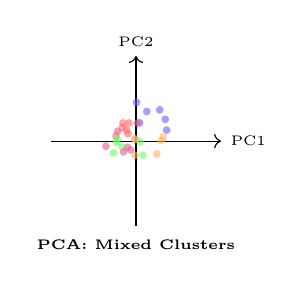
\begin{tikzpicture}[scale=0.6]
    % PCA axes
    \draw[->] (-1.8,0) -- (1.8,0) node[right] {\tiny PC1};
    \draw[->] (0,-1.8) -- (0,1.8) node[above] {\tiny PC2};
    
    % Overlapping clusters - PCA
    \foreach \x/\y/\c in {-0.4/0.4/red!60, 0.3/0.5/blue!60, -0.2/-0.3/green!60, 
                          0.3/-0.2/orange!60, -0.3/0.1/purple!60} {
        \foreach \i in {1,...,6} {
            \pgfmathsetmacro{\rx}{0.35*rand}
            \pgfmathsetmacro{\ry}{0.35*rand}
            \node[circle, fill=\c, inner sep=1pt, opacity=0.6] at (\x+\rx,\y+\ry) {};
        }
    }
    
    \node at (0,-2.2) {\tiny \textbf{PCA: Mixed Clusters}};
\end{tikzpicture}
\end{center}

\footnotesize
\textcolor{upcgray}{\textbf{Problems:}}
\begin{itemize}
    \tiny
    \item Classes overlap significantly
    \item Linear projection limitations
    \item Poor cluster separation
\end{itemize}
\end{column}

\begin{column}{0.48\textwidth}
\textbf{\color{upcblue}t-SNE on MNIST Digits}

\begin{center}
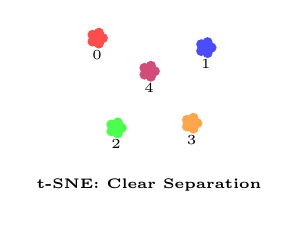
\begin{tikzpicture}[scale=0.6]
    % t-SNE well-separated clusters
    \foreach \x/\y/\c/\l in {-1.1/0.9/red!70/0, 1.2/0.7/blue!70/1, 
                              -0.7/-1/green!70/2, 0.9/-0.9/orange!70/3, 
                              0/0.2/purple!70/4} {
        % Tight cluster
        \foreach \i in {1,...,5} {
            \pgfmathsetmacro{\angle}{360*\i/5}
            \node[circle, fill=\c, inner sep=1.3pt] at ({\x+0.12*cos(\angle)},{\y+0.12*sin(\angle)}) {};
        }
        \node[circle, fill=\c, inner sep=1.3pt] at (\x,\y) {};
        \node at (\x,\y-0.35) {\tiny \l};
    }
    
    \node at (0,-2.2) {\tiny \textbf{t-SNE: Clear Separation}};
\end{tikzpicture}
\end{center}

\footnotesize
\textcolor{highlight}{\textbf{Advantages:}}
\begin{itemize}
    \tiny
    \item Distinct clusters
    \item Preserves local structure
    \item Reveals true relationships
\end{itemize}
\end{column}
\end{columns}

\vspace{0.15cm}
\begin{center}
\colorbox{upcblue!10}{
\begin{minipage}{0.8\textwidth}
\centering
\footnotesize\textit{``t-SNE focuses on preserving \textbf{local neighborhood structure}''}\\
\footnotesize\textit{Similar points in high-D $\rightarrow$ nearby points in low-D}
\end{minipage}
}
\end{center}
\end{frame}

% SLIDE 8: Lecture Outline (Aesthetic Revision)
\begin{frame}{Today's Journey: From Theory to Mastery}
\vspace{1cm} 
\centering
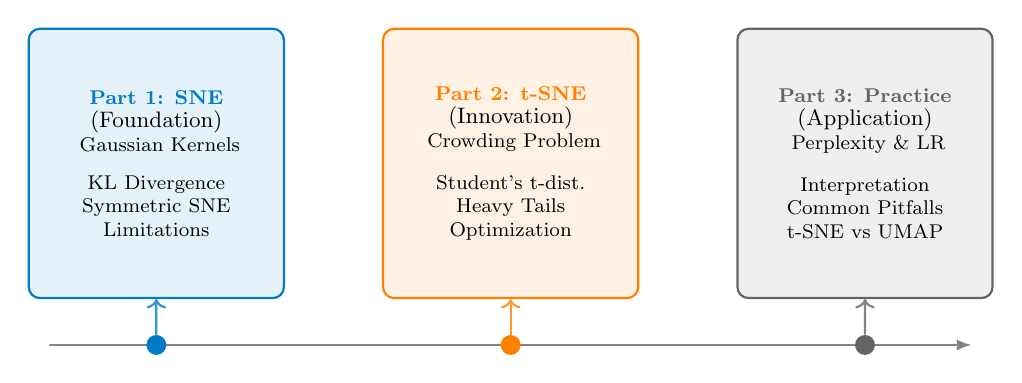
\begin{tikzpicture}[
    scale=0.9, transform shape,
    % Styles
    box/.style={
        draw, thick, rounded corners,
        minimum width=3.6cm, minimum height=3.8cm,
        align=center, font=\footnotesize,
        inner sep=5pt
    },
    point/.style={
        circle, fill, minimum size=8pt, inner sep=0pt
    },
    timeline/.style={
        -latex, thick, upcgray!80, line cap=round
    }
]

% The main timeline arrow
\draw[timeline] (-6.5,0) -- (6.5,0);

% Part 1: SNE
\node[point, fill=upcblue] (p1) at (-5,0) {};
\node[box, draw=upcblue, fill=upcblue!10, above=0.5cm of p1] (b1) {
    \textbf{\color{upcblue}Part 1: SNE} \\
    \small(Foundation) \\ \vspace{2mm}
    Gaussian Kernels \\
    KL Divergence \\
    Symmetric SNE \\
    Limitations
};
\draw[->, thick, upcblue!80] (p1.north) -- (b1.south);

% Part 2: t-SNE
\node[point, fill=highlight] (p2) at (0,0) {};
\node[box, draw=highlight, fill=highlight!10, above=0.5cm of p2] (b2) {
    \textbf{\color{highlight}Part 2: t-SNE} \\
    \small(Innovation) \\ \vspace{2mm}
    Crowding Problem \\
    Student's t-dist. \\
    Heavy Tails \\
    Optimization
};
\draw[->, thick, highlight!80] (p2.north) -- (b2.south);

% Part 3: Practice
\node[point, fill=upcgray] (p3) at (5,0) {};
\node[box, draw=upcgray, fill=upcgray!10, above=0.5cm of p3] (b3) {
    \textbf{\color{upcgray}Part 3: Practice} \\
    \small(Application) \\ \vspace{2mm}
    Perplexity \& LR \\
    Interpretation \\
    Common Pitfalls \\
    t-SNE vs UMAP
};
\draw[->, thick, upcgray!80] (p3.north) -- (b3.south);

\end{tikzpicture}
\end{frame}


% SLIDE 9: Let's Begin - The Core Idea
\begin{frame}{From Distances to Probabilities: The Core Idea}
\vspace{-0.2cm}

\begin{center}
\colorbox{upcblue!10}{
\begin{minipage}{0.85\textwidth}
\centering
\textbf{Central Insight:} Convert distances between points into probabilities\\
that represent neighborhood relationships
\end{minipage}
}
\end{center}

\vspace{0.3cm}
\begin{columns}[T]
\begin{column}{0.48\textwidth}
\textbf{\color{upcblue}Traditional Approach}
\vspace{0.2cm}

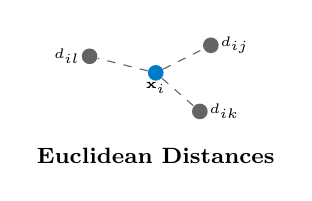
\begin{tikzpicture}[scale=0.7]
    % Distance-based
    \node[circle, fill=upcblue, inner sep=2pt] (c) at (0,0) {};
    \node[below] at (c) {\tiny $\mathbf{x}_i$};
    
    \node[circle, fill=upcgray, inner sep=2pt] (p1) at (1,0.5) {};
    \node[right] at (p1) {\tiny $d_{ij}$};
    
    \node[circle, fill=upcgray, inner sep=2pt] (p2) at (0.8,-0.7) {};
    \node[right] at (p2) {\tiny $d_{ik}$};
    
    \node[circle, fill=upcgray, inner sep=2pt] (p3) at (-1.2,0.3) {};
    \node[left] at (p3) {\tiny $d_{il}$};
    
    \draw[dashed, upcgray] (c) -- (p1);
    \draw[dashed, upcgray] (c) -- (p2);
    \draw[dashed, upcgray] (c) -- (p3);
    
    \node at (0,-1.5) {\footnotesize \textbf{Euclidean Distances}};
\end{tikzpicture}

\footnotesize
Problem: How to weight different distances?
\end{column}

\begin{column}{0.48\textwidth}
\textbf{\color{upcblue}SNE/t-SNE Approach}
\vspace{0.2cm}

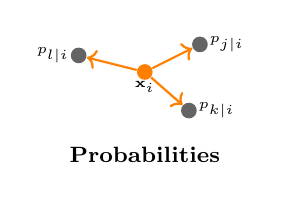
\begin{tikzpicture}[scale=0.7]
    % Probability-based
    \node[circle, fill=highlight, inner sep=2pt] (c) at (0,0) {};
    \node[below] at (c) {\tiny $\mathbf{x}_i$};
    
    \node[circle, fill=upcgray, inner sep=2pt] (p1) at (1,0.5) {};
    \node[right] at (p1) {\tiny $p_{j|i}$};
    
    \node[circle, fill=upcgray, inner sep=2pt] (p2) at (0.8,-0.7) {};
    \node[right] at (p2) {\tiny $p_{k|i}$};
    
    \node[circle, fill=upcgray, inner sep=2pt] (p3) at (-1.2,0.3) {};
    \node[left] at (p3) {\tiny $p_{l|i}$};
    
    \draw[->, highlight, thick] (c) -- (p1);
    \draw[->, highlight, thick] (c) -- (p2);
    \draw[->, highlight, thick] (c) -- (p3);
    
    \node at (0,-1.5) {\footnotesize \textbf{Probabilities}};
\end{tikzpicture}

\footnotesize
Solution: Probabilities naturally normalize!
\end{column}
\end{columns}

\vspace{0.3cm}
\begin{center}
\colorbox{highlight!20}{
\begin{minipage}{0.85\textwidth}
\centering
\footnotesize\textit{``What is the probability that point $i$ would pick point $j$ as its neighbor?''}
\end{minipage}
}
\end{center}
\end{frame}



% SLIDE 10: Part 1 Begins - SNE Foundations
\begin{frame}{Part 1: Stochastic Neighbor Embedding (SNE)}
\vspace{-0.2cm}

\begin{center}
\colorbox{upcblue!10}{
\begin{minipage}{0.85\textwidth}
\centering
\textbf{The Foundation:} Understanding the original SNE algorithm\\
before moving to t-SNE improvements
\end{minipage}
}
\end{center}

\vspace{0.3cm}
\begin{columns}[T]
\begin{column}{0.48\textwidth}
\textbf{\color{upcblue}What We'll Cover}
\vspace{0.2cm}

\begin{enumerate}
    \small
    \setlength\itemsep{0.3em}
    \item High-dimensional similarities
    \item Gaussian kernels
    \item Conditional probabilities
    \item Perplexity parameter
    \item Low-dimensional mapping
    \item KL divergence objective
    \item Gradient computation
\end{enumerate}
\end{column}

\begin{column}{0.48\textwidth}
\textbf{\color{upcblue}Key References}
\vspace{0.2cm}

\small
\textcolor{upcgray}{Original Paper:}\\
\footnotesize
Hinton \& Roweis (2002)\\
\textit{``Stochastic Neighbor Embedding''}\\
NIPS 2002

\vspace{0.3cm}
\textcolor{upcgray}{Mathematical Framework:}\\
\footnotesize
Building on MDS, Isomap, LLE\\
but with probabilistic approach

\vspace{0.3cm}
\begin{center}
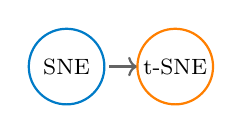
\begin{tikzpicture}[scale=0.6]
    \draw[thick, upcblue] (0,0) circle (0.8cm);
    \node at (0,0) {\footnotesize SNE};
    \draw[->, thick, upcgray] (0.9,0) -- (1.5,0);
    \draw[thick, highlight] (2.3,0) circle (0.8cm);
    \node at (2.3,0) {\footnotesize t-SNE};
\end{tikzpicture}
\end{center}
\end{column}
\end{columns}

\vspace{0.3cm}
\begin{center}
\colorbox{highlight!20}{
\begin{minipage}{0.85\textwidth}
\centering
\footnotesize\textit{``SNE converts high-dimensional Euclidean distances into}\\
\footnotesize\textit{conditional probabilities that represent similarities''}
\end{minipage}
}
\end{center}
\end{frame}


% SLIDE 11: High-Dimensional Similarity - Gaussian Kernels
\begin{frame}{High-Dimensional Similarity: Gaussian Kernels}
\vspace{-0.2cm}

\textbf{\color{upcblue}The Core Question:} How similar are two points in high-dimensional space?

\vspace{0.3cm}
\begin{columns}[T]
\begin{column}{0.5\textwidth}
\textbf{\color{upcblue}Gaussian Similarity}
\vspace{0.2cm}

\begin{center}
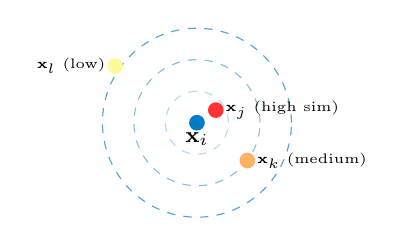
\begin{tikzpicture}[scale=0.8]
    % Central point
    \node[circle, fill=upcblue, inner sep=2pt] at (0,0) (xi) {};
    \node[below] at (xi) {\footnotesize $\mathbf{x}_i$};
    
    % Gaussian circles
    \draw[upcblue!30, dashed] (0,0) circle (0.5cm);
    \draw[upcblue!50, dashed] (0,0) circle (1cm);
    \draw[upcblue!70, dashed] (0,0) circle (1.5cm);
    
    % Nearby points
    \node[circle, fill=red!80, inner sep=2pt] at (0.3,0.2) (xj) {};
    \node[right] at (xj) {\tiny $\mathbf{x}_j$ (high sim)};
    
    \node[circle, fill=orange!60, inner sep=2pt] at (0.8,-0.6) (xk) {};
    \node[right] at (xk) {\tiny $\mathbf{x}_k$ (medium)};
    
    \node[circle, fill=yellow!40, inner sep=2pt] at (-1.3,0.9) (xl) {};
    \node[left] at (xl) {\tiny $\mathbf{x}_l$ (low)};
\end{tikzpicture}
\end{center}

\small
\textcolor{upcgray}{Similarity decreases with distance}\\
\textcolor{upcgray}{following Gaussian decay}
\end{column}

\begin{column}{0.5\textwidth}
\textbf{\color{upcblue}Mathematical Form}
\vspace{0.2cm}

Unnormalized similarity:
$$\text{sim}(i,j) = \exp\left(-\frac{\|\mathbf{x}_i - \mathbf{x}_j\|^2}{2\sigma_i^2}\right)$$

\vspace{0.3cm}
\textbf{Key Properties:}
\begin{itemize}
    \small
    \item Range: $(0, 1]$
    \item Max when $i = j$
    \item Smooth decay
    \item Point-specific $\sigma_i$
\end{itemize}

\vspace{0.2cm}
\small
\textcolor{highlight}{\textbf{Critical:}} $\sigma_i$ controls the\\
"neighborhood size" for point $i$
\end{column}
\end{columns}

\vspace{0.3cm}
\begin{center}
\colorbox{upcblue!10}{
\begin{minipage}{0.85\textwidth}
\centering
\footnotesize\textit{Reference: van der Maaten \& Hinton (2008), Equation 1}
\end{minipage}
}
\end{center}
\end{frame}


% SLIDE 12: High-Dimensional Similarity - The Formula
\begin{frame}{The Conditional Probability $p_{j|i}$}
\vspace{-0.3cm}

\begin{center}
\colorbox{upcblue!10}{
\begin{minipage}{0.85\textwidth}
\centering
\large
$$p_{j|i} = \frac{\exp(-\|\mathbf{x}_i - \mathbf{x}_j\|^2 / 2\sigma_i^2)}{\sum_{k \neq i} \exp(-\|\mathbf{x}_i - \mathbf{x}_k\|^2 / 2\sigma_i^2)}$$
\end{minipage}
}
\end{center}

\vspace{0.2cm}
\textbf{\color{upcblue}Breaking Down the Components:}

\vspace{0.15cm}
\begin{columns}[T]
\begin{column}{0.48\textwidth}
\textbf{Numerator:}
$$\exp\left(-\frac{\|\mathbf{x}_i - \mathbf{x}_j\|^2}{2\sigma_i^2}\right)$$

\footnotesize
\vspace{-0.1cm}
\begin{itemize}
    \setlength\itemsep{0.1em}
    \item $\|\mathbf{x}_i - \mathbf{x}_j\|^2$: Squared distance
    \item $\sigma_i^2$: Variance for point $i$
    \item Gaussian kernel at $\mathbf{x}_i$
\end{itemize}
\end{column}

\begin{column}{0.48\textwidth}
\textbf{Denominator:}
$$\sum_{k \neq i} \exp\left(-\frac{\|\mathbf{x}_i - \mathbf{x}_k\|^2}{2\sigma_i^2}\right)$$

\footnotesize
\vspace{-0.1cm}
\begin{itemize}
    \setlength\itemsep{0.1em}
    \item Sum over all other points
    \item Ensures $\sum_j p_{j|i} = 1$
    \item Makes it a probability
\end{itemize}
\end{column}
\end{columns}

\vspace{0.15cm}
\begin{center}
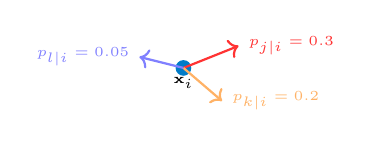
\begin{tikzpicture}[scale=0.7]
    % Visualization
    \node[circle, fill=upcblue, inner sep=2pt] at (0,0) (xi) {};
    \node[below] at (xi) {\tiny $\mathbf{x}_i$};
    
    % Probability arrows
    \draw[->, thick, red!80] (0,0) -- (1,0.4) node[right] {\tiny $p_{j|i} = 0.3$};
    \draw[->, thick, orange!60] (0,0) -- (0.7,-0.6) node[right] {\tiny $p_{k|i} = 0.2$};
    \draw[->, thick, blue!50] (0,0) -- (-0.8,0.2) node[left] {\tiny $p_{l|i} = 0.05$};
\end{tikzpicture}
\end{center}

\vspace{-0.1cm}
\begin{center}
\colorbox{highlight!20}{
\begin{minipage}{0.8\textwidth}
\centering
\tiny\textbf{Interpretation:} $p_{j|i}$ = probability that $i$ picks $j$ as neighbor
\end{minipage}
}
\end{center}
\end{frame}



% SLIDE 13: Perplexity - An Intuitive Bandwidth
\begin{frame}{Tuning Neighborhood Size: Perplexity}
\vspace{-0.2cm}

\textbf{\color{upcblue}The Problem:} How to choose $\sigma_i$ for each point?

\vspace{0.2cm}
\begin{center}
\colorbox{upcblue!10}{
\begin{minipage}{0.85\textwidth}
\centering
\textbf{Solution:} Use \textit{Perplexity} - a user-specified parameter that\\
indirectly sets $\sigma_i$ through binary search
\end{minipage}
}
\end{center}

\vspace{0.3cm}
\begin{columns}[T]
\begin{column}{0.48\textwidth}
\textbf{\color{upcblue}Definition}
\vspace{0.2cm}

$$\text{Perp}(P_i) = 2^{H(P_i)}$$

where Shannon entropy:
$$H(P_i) = -\sum_j p_{j|i} \log_2 p_{j|i}$$

\vspace{0.2cm}
\textbf{Interpretation:}\\
\footnotesize
Perplexity = effective number of neighbors

\vspace{0.2cm}
\textbf{Typical values:} 5-50
\end{column}

\begin{column}{0.48\textwidth}
\textbf{\color{upcblue}Binary Search for $\sigma_i$}
\vspace{0.2cm}

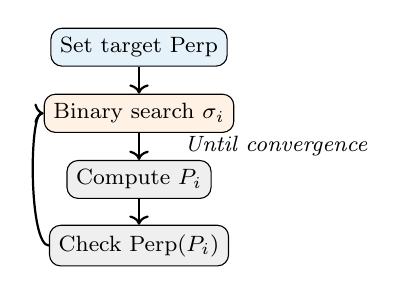
\begin{tikzpicture}[scale=0.7]
    % Flow diagram
    \node[draw, rounded corners, fill=upcblue!10] (start) at (0,0) {\footnotesize Set target Perp};
    \node[draw, rounded corners, fill=highlight!10] (search) at (0,-1.2) {\footnotesize Binary search $\sigma_i$};
    \node[draw, rounded corners, fill=upcgray!10] (compute) at (0,-2.4) {\footnotesize Compute $P_i$};
    \node[draw, rounded corners, fill=upcgray!10] (check) at (0,-3.6) {\footnotesize Check Perp$(P_i)$};
    
    \draw[->, thick] (start) -- (search);
    \draw[->, thick] (search) -- (compute);
    \draw[->, thick] (compute) -- (check);
    \draw[->, thick] (check.west) .. controls (-2,-3.6) and (-2,-1.2) .. (search.west);
    
    \node at (2.5,-1.8) {\footnotesize \textit{Until convergence}};
\end{tikzpicture}
\end{column}
\end{columns}

\vspace{0.2cm}
\begin{center}
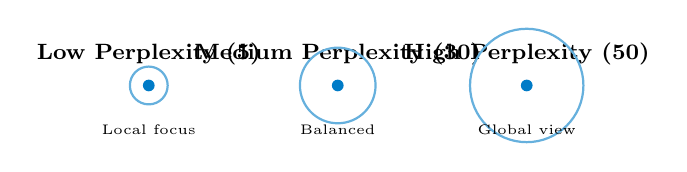
\begin{tikzpicture}[scale=0.8]
    % Visual comparison
    \node at (-3,0) {\footnotesize \textbf{Low Perplexity (5)}};
    \node[circle, fill=upcblue, inner sep=1.5pt] at (-3,-0.5) {};
    \draw[upcblue!60, thick] (-3,-0.5) circle (0.3cm);
    \node at (-3,-1.2) {\tiny Local focus};
    
    \node at (0,0) {\footnotesize \textbf{Medium Perplexity (30)}};
    \node[circle, fill=upcblue, inner sep=1.5pt] at (0,-0.5) {};
    \draw[upcblue!60, thick] (0,-0.5) circle (0.6cm);
    \node at (0,-1.2) {\tiny Balanced};
    
    \node at (3,0) {\footnotesize \textbf{High Perplexity (50)}};
    \node[circle, fill=upcblue, inner sep=1.5pt] at (3,-0.5) {};
    \draw[upcblue!60, thick] (3,-0.5) circle (0.9cm);
    \node at (3,-1.2) {\tiny Global view};
\end{tikzpicture}
\end{center}
\end{frame}




% SLIDE 14: Visualizing Perplexity's Effect
\begin{frame}{Perplexity in Action}
\vspace{-0.2cm}

\begin{center}
\textbf{\color{upcblue}How Perplexity Affects Point Neighborhoods}
\end{center}

\vspace{0.3cm}
\begin{columns}[T]
\begin{column}{0.48\textwidth}
\textbf{\color{upcblue}Dense Region}
\vspace{0.2cm}

\begin{center}
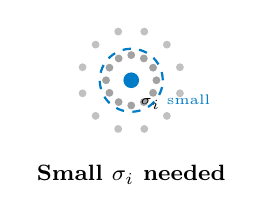
\begin{tikzpicture}[scale=0.8]
    % Dense cluster of points
    \node[circle, fill=upcblue, inner sep=2pt] at (0,0) {};
    \foreach \angle in {0,30,...,330} {
        \node[circle, fill=upcgray!60, inner sep=1pt] at ({0.4*cos(\angle)},{0.4*sin(\angle)}) {};
    }
    \foreach \angle in {15,45,...,345} {
        \node[circle, fill=upcgray!40, inner sep=1pt] at ({0.8*cos(\angle)},{0.8*sin(\angle)}) {};
    }
    
    % Gaussian curve
    \draw[upcblue, thick, dashed] (0,0) circle (0.5cm);
    \node at (0.7,-0.35) {\tiny $\sigma_i$ \textcolor{upcblue}{small}};
    
    \node at (0,-1.5) {\footnotesize \textbf{Small $\sigma_i$ needed}};
\end{tikzpicture}
\end{center}

\footnotesize
Many nearby points\\
$\rightarrow$ Narrow Gaussian\\
$\rightarrow$ Small $\sigma_i$ achieves target perplexity
\end{column}

\begin{column}{0.48\textwidth}
\textbf{\color{upcblue}Sparse Region}
\vspace{0.2cm}

\begin{center}
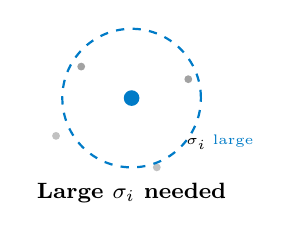
\begin{tikzpicture}[scale=0.8]
    % Sparse points
    \node[circle, fill=upcblue, inner sep=2pt] at (0,0) {};
    \node[circle, fill=upcgray!60, inner sep=1pt] at (0.9,0.3) {};
    \node[circle, fill=upcgray!60, inner sep=1pt] at (-0.8,0.5) {};
    \node[circle, fill=upcgray!40, inner sep=1pt] at (0.4,-1.1) {};
    \node[circle, fill=upcgray!40, inner sep=1pt] at (-1.2,-0.6) {};
    
    % Gaussian curve
    \draw[upcblue, thick, dashed] (0,0) circle (1.1cm);
    \node at (1.4,-0.7) {\tiny $\sigma_i$ \textcolor{upcblue}{large}};
    
    \node at (0,-1.5) {\footnotesize \textbf{Large $\sigma_i$ needed}};
\end{tikzpicture}
\end{center}

\footnotesize
Few nearby points\\
$\rightarrow$ Wide Gaussian\\
$\rightarrow$ Large $\sigma_i$ achieves target perplexity
\end{column}
\end{columns}

\vspace{0.3cm}
\begin{center}
\colorbox{highlight!20}{
\begin{minipage}{0.85\textwidth}
\centering
\footnotesize\textbf{Key Insight:} SNE automatically adapts to local data density\\
\footnotesize Dense regions get small $\sigma_i$, sparse regions get large $\sigma_i$
\end{minipage}
}
\end{center}

\vspace{0.2cm}
\begin{center}
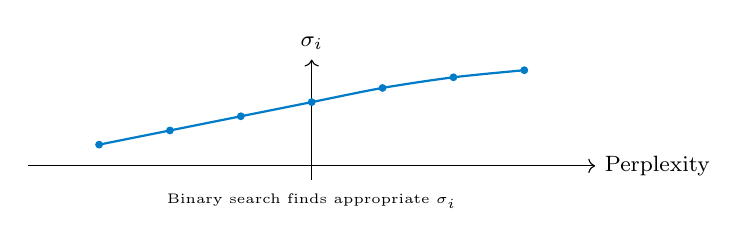
\begin{tikzpicture}[scale=0.9]
    % Perplexity effect visualization
    \draw[->] (-4,0) -- (4,0) node[right] {\footnotesize Perplexity};
    \draw[->] (0,-0.2) -- (0,1.5) node[above] {\footnotesize $\sigma_i$};
    
    % Points showing relationship
    \foreach \x/\y in {-3/0.3, -2/0.5, -1/0.7, 0/0.9, 1/1.1, 2/1.25, 3/1.35} {
        \node[circle, fill=upcblue, inner sep=1pt] at (\x,\y) {};
    }
    \draw[upcblue, thick] plot[smooth] coordinates {(-3,0.3) (-2,0.5) (-1,0.7) (0,0.9) (1,1.1) (2,1.25) (3,1.35)};
    
    \node at (0,-0.5) {\tiny Binary search finds appropriate $\sigma_i$};
\end{tikzpicture}
\end{center}
\end{frame}






% SLIDE 15: Low-Dimensional Similarity - Gaussian for SNE
\begin{frame}{Low-Dimensional Similarity ($q_{j|i}$): Standard Gaussians}
\vspace{-0.3cm}

\begin{center}
\colorbox{upcblue!10}{
\begin{minipage}{0.85\textwidth}
\centering
$$q_{j|i} = \frac{\exp(-\|\mathbf{y}_i - \mathbf{y}_j\|^2)}{\sum_{k \neq i} \exp(-\|\mathbf{y}_i - \mathbf{y}_k\|^2)}$$
\end{minipage}
}
\end{center}

\vspace{0.2cm}
\textbf{\color{upcblue}Key Differences from High-D:}

\begin{columns}[T]
\begin{column}{0.48\textwidth}
\textbf{Fixed Variance}

\begin{center}
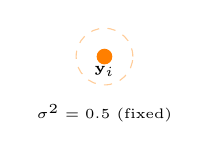
\begin{tikzpicture}[scale=0.6]
    \node[circle, fill=highlight, inner sep=2pt] at (0,0) {};
    \node[below] at (0,0) {\tiny $\mathbf{y}_i$};
    \draw[highlight!40, dashed] (0,0) circle (0.6cm);
    \node at (0,-1.2) {\tiny $\sigma^2 = 0.5$ (fixed)};
\end{tikzpicture}
\end{center}

\footnotesize
No point-specific $\sigma_i$\\
Often $\sigma^2 = 0.5$\\
Or absorbed into gradient
\end{column}

\begin{column}{0.48\textwidth}
\textbf{Why Fixed?}

\footnotesize
1. \textbf{Equal density:}\\
   Points equally dense in low-D\\
2. \textbf{Scale arbitrary:}\\
   Can rescale embedding\\
3. \textbf{Simplification:}\\
   Fewer parameters

\vspace{0.2cm}
\textcolor{highlight}{\textbf{Result:}} Simpler optimization
\end{column}
\end{columns}

\vspace{0.2cm}
\begin{center}
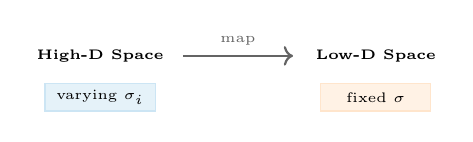
\begin{tikzpicture}[scale=0.7]
    \node at (-2.5,0) {\tiny \textbf{High-D Space}};
    \draw[upcblue!20, fill=upcblue!10] (-3.5,-0.5) rectangle (-1.5,-1);
    \node at (-2.5,-0.75) {\tiny varying $\sigma_i$};
    
    \draw[->, thick, upcgray] (-1,0) -- (1,0) node[midway, above] {\tiny map};
    
    \node at (2.5,0) {\tiny \textbf{Low-D Space}};
    \draw[highlight!20, fill=highlight!10] (1.5,-0.5) rectangle (3.5,-1);
    \node at (2.5,-0.75) {\tiny fixed $\sigma$};
\end{tikzpicture}
\end{center}
\end{frame}

% SLIDE 16: Measuring Mismatch - KL Divergence (Repaired and Enhanced)
\begin{frame}{Measuring Mismatch: Kullback-Leibler Divergence}
\vspace{-0.2cm}

% --- The KL Divergence Formula ---
\begin{center}
\colorbox{upcblue!10}{
\begin{minipage}{0.9\textwidth}
\centering
\small Intuition: The cost of encoding data from distribution $P$ using a code optimized for distribution $Q$.
$$ \text{KL}(P||Q) = \sum_{j} p_j \log\left(\frac{p_j}{q_j}\right) $$
\end{minipage}
}
\end{center}
\vspace{0.2cm}

% --- Columns for Properties and Penalty Visualization ---
\begin{columns}[T]
\begin{column}{0.48\textwidth}
\textbf{\color{upcblue}Key Properties}
\begin{itemize}
    \setlength\itemsep{0.3em}
    \item Always non-negative: $\text{KL}(P||Q) \ge 0$
    \item Zero if and only if $P=Q$
    \item \textbf{Not a distance metric} because it's \textbf{asymmetric}:
    \begin{itemize}
        \item[] $\text{KL}(P||Q) \neq \text{KL}(Q||P)$
    \end{itemize}
\end{itemize}

\vspace{0.1cm}
\colorbox{highlight!20}{
\begin{minipage}{0.9\linewidth}
\small
\textbf{SNE's Goal:} Minimize $\sum_i \text{KL}(P_i||Q_i)$, where $P_i$ are high-dim probabilities and $Q_i$ are low-dim probabilities.
\end{minipage}
}

\end{column}

\begin{column}{0.48\textwidth}
\textbf{\color{upcblue}Asymmetric Penalty}

\begin{center}
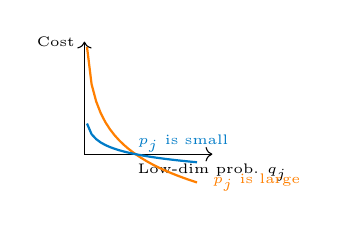
\begin{tikzpicture}[scale=0.65]
    % Axes
    \draw[->] (0,0) -- (2.5,0) node[below] {\tiny Low-dim prob. $q_j$};
    \draw[->] (0,0) -- (0,2.2) node[left] {\tiny Cost};
    
    % Plots of the cost term contribution: -p_j * log(q_j)
    \draw[highlight, thick, domain=0.05:2.2] plot (\x, {-0.7*ln(\x)}) node[right, font=\tiny, xshift=2pt] {$p_j$ is large};
    \draw[upcblue, thick, domain=0.05:2.2] plot (\x, {-0.2*ln(\x)}) node[above, font=\tiny, xshift=-5pt] {$p_j$ is small};
\end{tikzpicture}
\end{center}
\footnotesize
\textbf{Focus:} A large penalty is incurred for representing nearby points ($p_j$ large) with distant map points ($q_j$ small).

\end{column}
\end{columns}
\vspace{0.2cm}

% --- Visual Summary of Penalties ---
\begin{center}
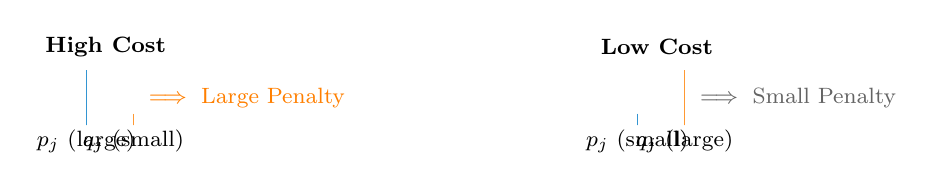
\begin{tikzpicture}[
    bar/.style={fill, minimum width=0.25cm},
    label/.style={font=\footnotesize}
]
    % Case 1: High Cost
    \begin{scope}[xshift=-3.5cm]
        \node[label, align=center] at (0.25, 1) {\textbf{High Cost}};
        % p_j is large
        \draw[bar, upcblue!80, minimum height=0.7cm] (0,0) -- (0,0.7);
        \node[label] at (0, -0.2) {$p_j$ (large)};
        % q_j is small
        \draw[bar, highlight!80, minimum height=0.15cm] (0.6,0) -- (0.6,0.15);
        \node[label] at (0.6, -0.2) {$q_j$ (small)};
        
        \node[label, color=highlight] at (2, 0.35) {$\implies$ Large Penalty};
    \end{scope}

    % Case 2: Low Cost
    \begin{scope}[xshift=3.5cm]
        \node[label, align=center] at (0.25, 1) {\textbf{Low Cost}};
        % p_j is small
        \draw[bar, upcblue!80, minimum height=0.15cm] (0,0) -- (0,0.15);
        \node[label] at (0, -0.2) {$p_j$ (small)};
        % q_j is large
        \draw[bar, highlight!80, minimum height=0.7cm] (0.6,0) -- (0.6,0.7);
        \node[label] at (0.6, -0.2) {$q_j$ (large)};
        
        \node[label, color=upcgray] at (2, 0.35) {$\implies$ Small Penalty};
    \end{scope}
\end{tikzpicture}
\end{center}
\end{frame}



% SLIDE 17: SNE's Cost Function
\begin{frame}{SNE Cost Function: C(Y)}
\vspace{-0.2cm}

\begin{center}
\colorbox{upcblue!10}{
\begin{minipage}{0.85\textwidth}
\centering
\large
$$C(Y) = \sum_{i=1}^{n} \text{KL}(P_i || Q_i) = \sum_i \sum_j p_{j|i} \log \frac{p_{j|i}}{q_{j|i}}$$
\end{minipage}
}
\end{center}

\vspace{0.3cm}
\textbf{\color{upcblue}Understanding the Cost:}

\begin{columns}[T]
\begin{column}{0.48\textwidth}
\textbf{What We Minimize}
\vspace{0.1cm}

\footnotesize
Sum over all points $i$:\\
Each $i$ has its own distribution $P_i$\\
We want $Q_i$ to match $P_i$

\vspace{0.2cm}
\begin{center}
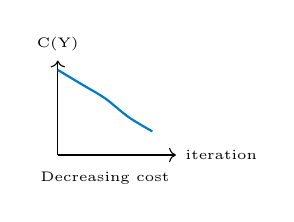
\begin{tikzpicture}[scale=0.6]
    \draw[->] (0,0) -- (2.5,0) node[right] {\tiny iteration};
    \draw[->] (0,0) -- (0,2) node[above] {\tiny C(Y)};
    
    \draw[upcblue, thick] plot[smooth] coordinates {(0,1.8) (0.5,1.5) (1,1.2) (1.5,0.8) (2,0.5)};
    \node at (1,-0.5) {\tiny Decreasing cost};
\end{tikzpicture}
\end{center}
\end{column}

\begin{column}{0.48\textwidth}
\textbf{Asymmetric Penalties}
\vspace{0.1cm}

\begin{center}

\begin{tikzpicture}[scale=0.5]
    % Nearby points
    \node[circle, fill=upcblue, inner sep=1pt] at (0,1) {};
    \node[circle, fill=upcblue, inner sep=1pt] at (0.3,1.2) {};
    \draw[<->, red, thick] (0.1,1.1) -- (0.2,1.1);
    \node at (0.15,0.7) {\tiny Must stay close};
    
    % Distant points
    \node[circle, fill=upcgray, inner sep=1pt] at (2,1) {};
    \node[circle, fill=upcgray, inner sep=1pt] at (2.3,0.8) {};
    \draw[<->, orange, dashed] (2.1,0.9) -- (2.2,0.9);
    \node at (2.15,0.5) {\tiny Can be flexible};
\end{tikzpicture}
\end{center}

\footnotesize
\textcolor{red}{High penalty:}\\
Similar points mapped far\\
\textcolor{orange}{Low penalty:}\\
Distant points mapped close
\end{column}
\end{columns}

\vspace{0.3cm}
\begin{center}
\colorbox{highlight!20}{
\begin{minipage}{0.85\textwidth}
\centering
\footnotesize\textbf{Result:} SNE preserves local neighborhoods at the expense of global structure
\end{minipage}
}
\end{center}

\vspace{0.2cm}
\begin{center}
\footnotesize
\textit{Reference: Hinton \& Roweis (2002), van der Maaten \& Hinton (2008) Eq. 3}
\end{center}
\end{frame}

% SLIDE 18: The Asymmetry and Local Focus of SNE
\begin{frame}{What Does SNE Prioritize?}
\vspace{-0.2cm}

\textbf{\color{upcblue}The Asymmetry of KL Divergence in Action}

\vspace{0.3cm}
\begin{center}
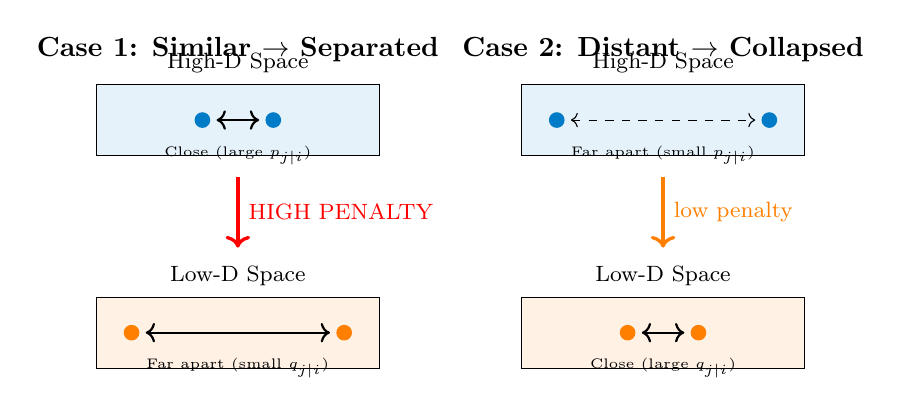
\begin{tikzpicture}[scale=0.9]
    % Case 1: Similar points separated
    \node at (-3,2) {\textbf{Case 1: Similar $\rightarrow$ Separated}};
    
    % High-D space
    \draw[fill=upcblue!10] (-5,0.5) rectangle (-1,1.5);
    \node at (-3,1.8) {\footnotesize High-D Space};
    \node[circle, fill=upcblue, inner sep=2pt] at (-3.5,1) {};
    \node[circle, fill=upcblue, inner sep=2pt] at (-2.5,1) {};
    \draw[<->, thick] (-3.3,1) -- (-2.7,1);
    \node at (-3,0.5) {\tiny Close (large $p_{j|i}$)};
    
    % Arrow down
    \draw[->, red, very thick] (-3,0.2) -- (-3,-0.8) node[midway, right] {\footnotesize\textcolor{red}{HIGH PENALTY}};
    
    % Low-D space
    \draw[fill=highlight!10] (-5,-2.5) rectangle (-1,-1.5);
    \node at (-3,-1.2) {\footnotesize Low-D Space};
    \node[circle, fill=highlight, inner sep=2pt] at (-4.5,-2) {};
    \node[circle, fill=highlight, inner sep=2pt] at (-1.5,-2) {};
    \draw[<->, thick] (-4.3,-2) -- (-1.7,-2);
    \node at (-3,-2.5) {\tiny Far apart (small $q_{j|i}$)};
    
    % Case 2: Distant points collapsed
    \node at (3,2) {\textbf{Case 2: Distant $\rightarrow$ Collapsed}};
    
    % High-D space
    \draw[fill=upcblue!10] (1,0.5) rectangle (5,1.5);
    \node at (3,1.8) {\footnotesize High-D Space};
    \node[circle, fill=upcblue, inner sep=2pt] at (1.5,1) {};
    \node[circle, fill=upcblue, inner sep=2pt] at (4.5,1) {};
    \draw[<->, dashed] (1.7,1) -- (4.3,1);
    \node at (3,0.5) {\tiny Far apart (small $p_{j|i}$)};
    
    % Arrow down
    \draw[->, orange, very thick] (3,0.2) -- (3,-0.8) node[midway, right] {\footnotesize\textcolor{orange}{low penalty}};
    
    % Low-D space
    \draw[fill=highlight!10] (1,-2.5) rectangle (5,-1.5);
    \node at (3,-1.2) {\footnotesize Low-D Space};
    \node[circle, fill=highlight, inner sep=2pt] at (2.5,-2) {};
    \node[circle, fill=highlight, inner sep=2pt] at (3.5,-2) {};
    \draw[<->, thick] (2.7,-2) -- (3.3,-2);
    \node at (3,-2.5) {\tiny Close (large $q_{j|i}$)};
\end{tikzpicture}
\end{center}

\vspace{0.3cm}
\begin{center}
\colorbox{upcblue!10}{
\begin{minipage}{0.85\textwidth}
\centering
\footnotesize\textbf{Key Insight:} SNE strongly preserves local neighborhoods (Case 1)\\
\footnotesize but allows distant points to collapse (Case 2)
\end{minipage}
}
\end{center}
\end{frame}


% SLIDE 19: Deriving the Gradient (Part 1)
\begin{frame}{Optimizing SNE: The Gradient $\frac{\partial C}{\partial \mathbf{y}_i}$}
\vspace{-0.2cm}

\begin{center}
\colorbox{upcblue!10}{
\begin{minipage}{0.85\textwidth}
\centering
\textbf{Gradient Descent:} Update positions to minimize cost\\
$$\mathbf{y}_i^{(t+1)} = \mathbf{y}_i^{(t)} - \eta \frac{\partial C}{\partial \mathbf{y}_i}$$
\end{minipage}
}
\end{center}

\vspace{0.3cm}
\textbf{\color{upcblue}The SNE Gradient Formula:}

$$\frac{\partial C}{\partial \mathbf{y}_i} = 2 \sum_{j=1}^{n} (p_{ij} - q_{ij} + p_{ji} - q_{ji})(\mathbf{y}_i - \mathbf{y}_j)$$

\vspace{0.2cm}
\begin{columns}[T]
\begin{column}{0.48\textwidth}
\textbf{Key Components}
\vspace{0.1cm}

\footnotesize
\textbf{Force terms:}\\
$(p_{ij} - q_{ij})$: Mismatch from $i$ to $j$\\
$(p_{ji} - q_{ji})$: Mismatch from $j$ to $i$\\

\vspace{0.2cm}
\textbf{Direction:}\\
$(\mathbf{y}_i - \mathbf{y}_j)$: Vector from $j$ to $i$
\end{column}

\begin{column}{0.48\textwidth}
\textbf{Derivation Steps}
\vspace{0.1cm}

\footnotesize
1. Start with KL divergence\\
2. Apply chain rule\\
3. Differentiate w.r.t. $\mathbf{y}_i$\\
4. Account for asymmetry\\
5. Simplify terms

\vspace{0.2cm}
\textit{Full derivation in van der Maaten \& Hinton (2008), Section 2}
\end{column}
\end{columns}

\vspace{0.3cm}
\begin{center}
\colorbox{highlight!20}{
\begin{minipage}{0.85\textwidth}
\centering
\footnotesize\textbf{Note:} The asymmetric nature requires considering both $p_{ij}$ and $p_{ji}$
\end{minipage}
}
\end{center}
\end{frame}

% SLIDE 20: Deriving the Gradient (Part 2: Intuition)
\begin{frame}{Gradient Intuition: Forces at Play}
\vspace{-0.2cm}

\begin{center}
\textbf{\color{upcblue}The Gradient as a System of Forces}
\end{center}

\vspace{0.3cm}
\begin{center}
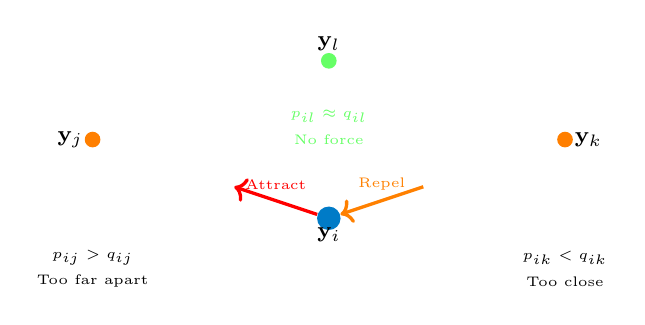
\begin{tikzpicture}[scale=1.0]
    % Central point
    \node[circle, fill=upcblue, inner sep=3pt] at (0,0) (yi) {};
    \node[below] at (yi) {\footnotesize $\mathbf{y}_i$};
    
    % Case 1: Attraction (p > q)
    \node[circle, fill=highlight, inner sep=2pt] at (-3,1) (yj1) {};
    \node[left] at (yj1) {\footnotesize $\mathbf{y}_j$};
    \draw[->, red, very thick] (yi) -- (-1.2,0.4) node[midway, above] {\tiny Attract};
    \node at (-3,-0.5) {\tiny $p_{ij} > q_{ij}$};
    \node at (-3,-0.8) {\tiny Too far apart};
    
    % Case 2: Repulsion (p < q)
    \node[circle, fill=highlight, inner sep=2pt] at (3,1) (yj2) {};
    \node[right] at (yj2) {\footnotesize $\mathbf{y}_k$};
    \draw[<-, orange, very thick] (yi) -- (1.2,0.4) node[midway, above] {\tiny Repel};
    \node at (3,-0.5) {\tiny $p_{ik} < q_{ik}$};
    \node at (3,-0.8) {\tiny Too close};
    
    % Balanced case
    \node[circle, fill=green!60, inner sep=2pt] at (0,2) (yj3) {};
    \node[above] at (yj3) {\footnotesize $\mathbf{y}_l$};
    \node[green!60] at (0,1.3) {\tiny $p_{il} \approx q_{il}$};
    \node[green!60] at (0,1) {\tiny No force};
\end{tikzpicture}
\end{center}

\vspace{0.3cm}
\begin{columns}[T]
\begin{column}{0.48\textwidth}
\begin{center}
\colorbox{red!10}{
\begin{minipage}{0.9\columnwidth}
\centering
\textbf{Attractive Force}\\
\footnotesize
When $p_{ij} > q_{ij}$:\\
Points should be closer\\
$\Rightarrow$ Pull together
\end{minipage}
}
\end{center}
\end{column}

\begin{column}{0.48\textwidth}
\begin{center}
\colorbox{orange!10}{
\begin{minipage}{0.9\columnwidth}
\centering
\textbf{Repulsive Force}\\
\footnotesize
When $p_{ij} < q_{ij}$:\\
Points are too close\\
$\Rightarrow$ Push apart
\end{minipage}
}
\end{center}
\end{column}
\end{columns}

\vspace{0.3cm}
\begin{center}
\colorbox{upcblue!10}{
\begin{minipage}{0.85\textwidth}
\centering
\footnotesize\textbf{Equilibrium:} Forces balance when $p_{ij} = q_{ij}$ for all pairs
\end{minipage}
}
\end{center}
\end{frame}
\end{document}